\documentclass[10pt]{article}
\usepackage{PlantillaCat}

\usepackage{amsmath}
\usepackage{tikz}
\usepackage{mathdots}
\usepackage{yhmath}
\usepackage{cancel}
\usepackage{color}
\usepackage{siunitx}
\usepackage{array}
\usepackage{multirow}
\usepackage{amssymb}
%\usepackage{gensymb}
\usepackage{tabularx}
\usepackage{booktabs}
\usetikzlibrary{fadings}

\title{Problemes de teoria de grafs}
\author{Aleix Torres i Camps}
\date{2019}


\begin{document}
\maketitle

\maketitle
\section{Nocions bàsiques}
En aquest apartat apareixen problemes relacionats amb les nocions bàsiques de connexió i distancia. A més, de problemes vinculats amb les formes matricials d'un graf. \\ \\

\large
\textsl{\textbf{Problema 1:} El nombre de vèrtexs de grau senar en un graf $G = (V, E)$ és parell.} \\ \\
\textbf{Solució:} \\
\normalsize
Aquest problema és el clàssic \textit{lema de les encaixades}, co\lgem orari de la següent fórmula (que va bé recordar).
$$
\sum_{u\in V} d(v) = 2 |E|
$$
En paraules diu que la suma dels graus del vèrtexs és igual a dos cops el nombre d'arestes. Aquest fet és evident perquè cada aresta és adjacent a exactament dos vértexs, quan sumem els graus la comptarem dues vegades. Ara, el problema ens motiva a distingir entre vèrtexs de grau senar i de grau parell. Siguin $U_1$ els vèrtexs de grau senar i $U_2$ els vértexs de grau parell ($V = U_1 \cupdot U_2$). La fórmula es pot escriure com:
$$
\sum_{u\in U_1} d(u) = 2 |E| - \sum_{u\in U_2} d(u)
$$
On a la dreta només apareixen termes parells, per tant el resultat és parell. I a l'esquerra hi ha una suma de $|U_1|$ termes senars. Sabent que aquesta ha de ser parell, n'hi ha d'haver un nombre parell. És a dir, $|U_1|$ és parell, que és el que voliem veure. \\ \\

\large
\textsl{\textbf{Problema 2:} Qualsevol graf amb $n\geq2$ vèrtexs, en té dos del mateix grau.} \\ \\
\textbf{Solució:} \\
\normalsize
El conjunt de possibles graus d'un graf de $n$ vèrtexs és subconjunt de $\{0,1,2,...,n-1\}$ (de cardinal $n$), ja que cada vèrtexs pot no tenir cap aresta o tenir-ne alguna fins arribar al màxim que seria ser adjacent amb els altres $n-1$ vèrtexs. Tot i així, en un graf no hi pot haver alhora un vèrtex de grau 0 (no és adjacent amb cap altre) i un vèrtex de grau $n-1$ (és adjacent amb tots els altres). Per tant, hi ha, com a molt, $n-1$ possibles graus diferents en un graf de $n$ vèrtexs. Aleshores, pel \textsl{Principi del Colomar}, existeixen dos vèrtexs que tenen el mateix grau, que és el que voliem demostrar. \\ \\

\large
\textsl{\textbf{Problema 3:} Quants grafs hi ha de 4 vèrtexs i 3 arestes? Quants n'hi ha no isomorfs?} \\ \\
\textbf{Solució:} \\
\normalsize
Anem a veure primer que el nombre de grafs amb $n$ vèrtexs i $m$ arestes és ${{n}\choose{2}}\choose{m}$. Això es deu al fet que les arestes d'un graf $G=(V, E)$ d'ordre $n$ (és a dir, $|V|=n$) és subconjunt de ${V}\choose{2}$ i per cada subconjunt $E$ d'arestes el graf és diferent i no n'hi ha més a part d'aquests. Si fixem que $|E| = m$, equival a dir que dels ${V}\choose{2}$ se'n trien $m$. D'on surt que els nombre de grafs d'ordre $n$ i mida $m$ és ${{n}\choose{2}}\choose{m}$. Pel cas $n=4$ i $m=3$, n'hi ha ${{{4}\choose{2}}\choose{3}} = {{6}\choose{3}} = 20$. \\ \\
En general, és difícil trobar tots els grafs no isomors de $n$ vèrtexs i $m$ arestes. Però per casos petits és pot fer, per $n=4$ i $m=3$ tenim:

\tikzset{every picture/.style={line width=0.75pt}} %set default line width to 0.75pt

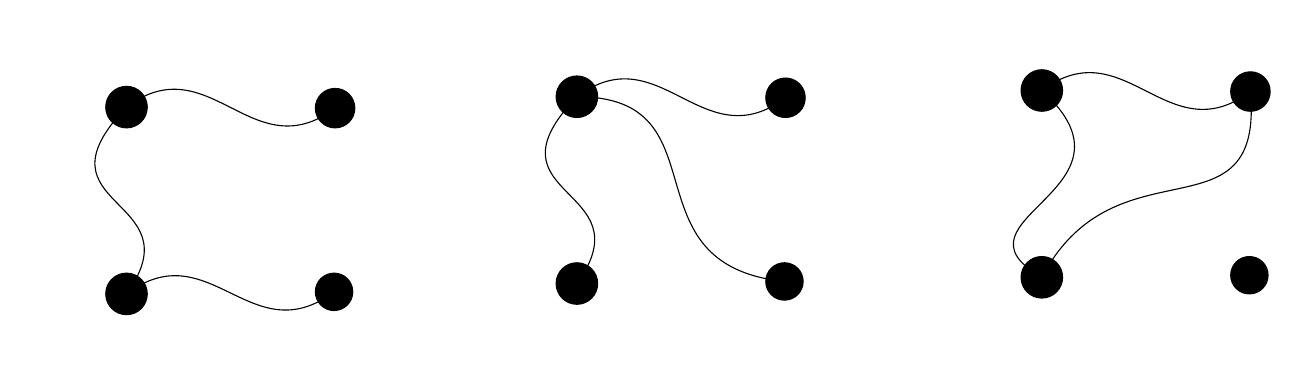
\begin{tikzpicture}[x=0.75pt,y=0.75pt,yscale=-1,xscale=1]
%uncomment if require: \path (0,200.1999969482422); %set diagram left start at 0, and has height of 200.1999969482422

%Shape: Circle [id:dp3740394366196229]
\draw  [fill={rgb, 255:red, 0; green, 0; blue, 0 }  ,fill opacity=1 ] (56.3,70.3) .. controls (56.3,64.78) and (60.78,60.3) .. (66.3,60.3) .. controls (71.82,60.3) and (76.3,64.78) .. (76.3,70.3) .. controls (76.3,75.82) and (71.82,80.3) .. (66.3,80.3) .. controls (60.78,80.3) and (56.3,75.82) .. (56.3,70.3) -- cycle ;
%Shape: Circle [id:dp5695258199560307]
\draw  [fill={rgb, 255:red, 0; green, 0; blue, 0 }  ,fill opacity=1 ] (56.3,160.3) .. controls (56.3,154.78) and (60.78,150.3) .. (66.3,150.3) .. controls (71.82,150.3) and (76.3,154.78) .. (76.3,160.3) .. controls (76.3,165.82) and (71.82,170.3) .. (66.3,170.3) .. controls (60.78,170.3) and (56.3,165.82) .. (56.3,160.3) -- cycle ;
%Shape: Circle [id:dp5288581861029809]
\draw  [fill={rgb, 255:red, 0; green, 0; blue, 0 }  ,fill opacity=1 ] (157.3,70.8) .. controls (157.3,65.55) and (161.55,61.3) .. (166.8,61.3) .. controls (172.05,61.3) and (176.3,65.55) .. (176.3,70.8) .. controls (176.3,76.05) and (172.05,80.3) .. (166.8,80.3) .. controls (161.55,80.3) and (157.3,76.05) .. (157.3,70.8) -- cycle ;
%Shape: Circle [id:dp6389645046522594]
\draw  [fill={rgb, 255:red, 0; green, 0; blue, 0 }  ,fill opacity=1 ] (157.3,159.3) .. controls (157.3,154.33) and (161.33,150.3) .. (166.3,150.3) .. controls (171.27,150.3) and (175.3,154.33) .. (175.3,159.3) .. controls (175.3,164.27) and (171.27,168.3) .. (166.3,168.3) .. controls (161.33,168.3) and (157.3,164.27) .. (157.3,159.3) -- cycle ;
%Curve Lines [id:da6021535459876024]
\draw    (66.3,70.3) .. controls (106.3,40.3) and (126.8,100.8) .. (166.8,70.8) ;


%Curve Lines [id:da5092091577079525]
\draw    (66.3,70.3) .. controls (18.95,119.65) and (100.3,113) .. (66.3,160.3) ;


%Curve Lines [id:da3802564061308329]
\draw    (66.3,160.3) .. controls (106.3,130.3) and (126.3,189.3) .. (166.3,159.3) ;


%Shape: Circle [id:dp8762376830880074]
\draw  [fill={rgb, 255:red, 0; green, 0; blue, 0 }  ,fill opacity=1 ] (273.3,65.3) .. controls (273.3,59.78) and (277.78,55.3) .. (283.3,55.3) .. controls (288.82,55.3) and (293.3,59.78) .. (293.3,65.3) .. controls (293.3,70.82) and (288.82,75.3) .. (283.3,75.3) .. controls (277.78,75.3) and (273.3,70.82) .. (273.3,65.3) -- cycle ;
%Shape: Circle [id:dp8446916081960136]
\draw  [fill={rgb, 255:red, 0; green, 0; blue, 0 }  ,fill opacity=1 ] (273.3,155.3) .. controls (273.3,149.78) and (277.78,145.3) .. (283.3,145.3) .. controls (288.82,145.3) and (293.3,149.78) .. (293.3,155.3) .. controls (293.3,160.82) and (288.82,165.3) .. (283.3,165.3) .. controls (277.78,165.3) and (273.3,160.82) .. (273.3,155.3) -- cycle ;
%Shape: Circle [id:dp21111036017806417]
\draw  [fill={rgb, 255:red, 0; green, 0; blue, 0 }  ,fill opacity=1 ] (374.3,65.8) .. controls (374.3,60.55) and (378.55,56.3) .. (383.8,56.3) .. controls (389.05,56.3) and (393.3,60.55) .. (393.3,65.8) .. controls (393.3,71.05) and (389.05,75.3) .. (383.8,75.3) .. controls (378.55,75.3) and (374.3,71.05) .. (374.3,65.8) -- cycle ;
%Shape: Circle [id:dp9798289634646031]
\draw  [fill={rgb, 255:red, 0; green, 0; blue, 0 }  ,fill opacity=1 ] (374.3,154.3) .. controls (374.3,149.33) and (378.33,145.3) .. (383.3,145.3) .. controls (388.27,145.3) and (392.3,149.33) .. (392.3,154.3) .. controls (392.3,159.27) and (388.27,163.3) .. (383.3,163.3) .. controls (378.33,163.3) and (374.3,159.27) .. (374.3,154.3) -- cycle ;
%Curve Lines [id:da5865000910016449]
\draw    (283.3,65.3) .. controls (323.3,35.3) and (343.8,95.8) .. (383.8,65.8) ;


%Curve Lines [id:da8071467440237363]
\draw    (283.3,65.3) .. controls (235.95,114.65) and (317.3,108) .. (283.3,155.3) ;


%Curve Lines [id:da5176040958693464]
\draw    (283.3,65.3) .. controls (355.3,65.2) and (305.3,146.2) .. (383.3,154.3) ;


%Shape: Circle [id:dp4622247399442818]
\draw  [fill={rgb, 255:red, 0; green, 0; blue, 0 }  ,fill opacity=1 ] (497.3,62.3) .. controls (497.3,56.78) and (501.78,52.3) .. (507.3,52.3) .. controls (512.82,52.3) and (517.3,56.78) .. (517.3,62.3) .. controls (517.3,67.82) and (512.82,72.3) .. (507.3,72.3) .. controls (501.78,72.3) and (497.3,67.82) .. (497.3,62.3) -- cycle ;
%Shape: Circle [id:dp8860820304788772]
\draw  [fill={rgb, 255:red, 0; green, 0; blue, 0 }  ,fill opacity=1 ] (497.3,152.3) .. controls (497.3,146.78) and (501.78,142.3) .. (507.3,142.3) .. controls (512.82,142.3) and (517.3,146.78) .. (517.3,152.3) .. controls (517.3,157.82) and (512.82,162.3) .. (507.3,162.3) .. controls (501.78,162.3) and (497.3,157.82) .. (497.3,152.3) -- cycle ;
%Shape: Circle [id:dp044109299678755765]
\draw  [fill={rgb, 255:red, 0; green, 0; blue, 0 }  ,fill opacity=1 ] (598.3,62.8) .. controls (598.3,57.55) and (602.55,53.3) .. (607.8,53.3) .. controls (613.05,53.3) and (617.3,57.55) .. (617.3,62.8) .. controls (617.3,68.05) and (613.05,72.3) .. (607.8,72.3) .. controls (602.55,72.3) and (598.3,68.05) .. (598.3,62.8) -- cycle ;
%Shape: Circle [id:dp980909117730919]
\draw  [fill={rgb, 255:red, 0; green, 0; blue, 0 }  ,fill opacity=1 ] (598.3,151.3) .. controls (598.3,146.33) and (602.33,142.3) .. (607.3,142.3) .. controls (612.27,142.3) and (616.3,146.33) .. (616.3,151.3) .. controls (616.3,156.27) and (612.27,160.3) .. (607.3,160.3) .. controls (602.33,160.3) and (598.3,156.27) .. (598.3,151.3) -- cycle ;
%Curve Lines [id:da18917831789422146]
\draw    (507.3,62.3) .. controls (547.3,32.3) and (567.8,92.8) .. (607.8,62.8) ;


%Curve Lines [id:da2577483107062264]
\draw    (507.3,62.3) .. controls (560.3,110.2) and (458.3,124.2) .. (507.3,152.3) ;


%Curve Lines [id:da880150623982469]
\draw    (507.3,152.3) .. controls (543.3,84.2) and (614.3,136.2) .. (607.8,62.8) ;


\end{tikzpicture}\\
Primer distingim entre que el graf sigui connex o no. Si no és connex l'única possibilitat és que tingui només dues components connexes. Una amb tres vèrtexs i tres arestes, i l'altre un vèrtex aïllat (això dona el tercer de la imatge). Després, pel cas connex, fem servir que necessàriament un vèrtex té almenys grau 2 (dalt esquerra amb dalt dreta i baix esquerra). Falta per determinar una aresta que ha de ser adjacent amb el vèrtex no connex i unir-lo amb un dels altres tres, dos d'ells donen el mateix graf isomorf per tant només compten per un. Així que si el graf és connex només hi ha dos casos, el camí (el primer) i l'estrella (el segon). \\ \\

\large
\textsl{\textbf{Problema 4:} Siguin $a_n$ el nombre de grafs d'ordre $n$ i $b_n$ el nombre de grafs no isomorfs d'ordre $n$. Proveu que $\log_2 a_n = n^2/2 + \mathcal{O}(n)$ i $\log_2 b_n = n^2/2+\mathcal{O}(n\log n)$. En particular, $\log b_n \sim \log a_n$, ($n\rightarrow \infty$).} \\ \\
\textbf{Solució:} \\
\normalsize
Sabem que hi ha $2^{{n}\choose{2}}$ grafs d'ordre $n$. Perquè per a cada dos vèrtexs pot haver-hi o no aresta. Llavors, $\log_2 a_n = {{n}\choose{2}} = n^2/2 + \mathcal{O}(n)$. Ara, $b_n$ no el podem calcular explícitament però sí donar una fita, de fet ja tenim una fita superior que és $a_n$. Podem deduir una cota inferiorment de $b_n$ de la següent manera. Dos grafs són isomorfs si hi ha una permutació dels vèrtexs que dona el mateix graf, però no totes les permutacions són vàlides. Per tant, $b_n\geq \frac{2^{{n}\choose{2}}}{n!}$, aixó assegura que $\log b_n = n^2/2 + \mathcal{O}(\log n!)$. Com $\mathcal{O}(\log n!)=\mathcal{O}(n\log n)$, hem obtingut el que voliem. La segona part, es demostra directament de les fórmules que ja hem deduit. \\ \\

\large
\textsl{\textbf{Problema 4:}} \\ \\
\textbf{Solució:} \\
\normalsize

\large
\textsl{\textbf{Problema 4:}} \\ \\
\textbf{Solució:} \\
\normalsize

\large
\textsl{\textbf{Problema 4:}} \\ \\
\textbf{Solució:} \\
\normalsize

\large
\textsl{\textbf{Problema 4:}} \\ \\
\textbf{Solució:} \\
\normalsize
\end{document} 